\chapter{Memory Stage}
\label{chp:memory_stage}
The memory stage allows to perform operations with the memory, the DRAM in this case, in order to load or store a value from/to the memory respectively. The figure \ref{fig:mem_stage} shows the Memory Stage of the DLX pipeline.

\begin{figure}[H]   
	\centering
	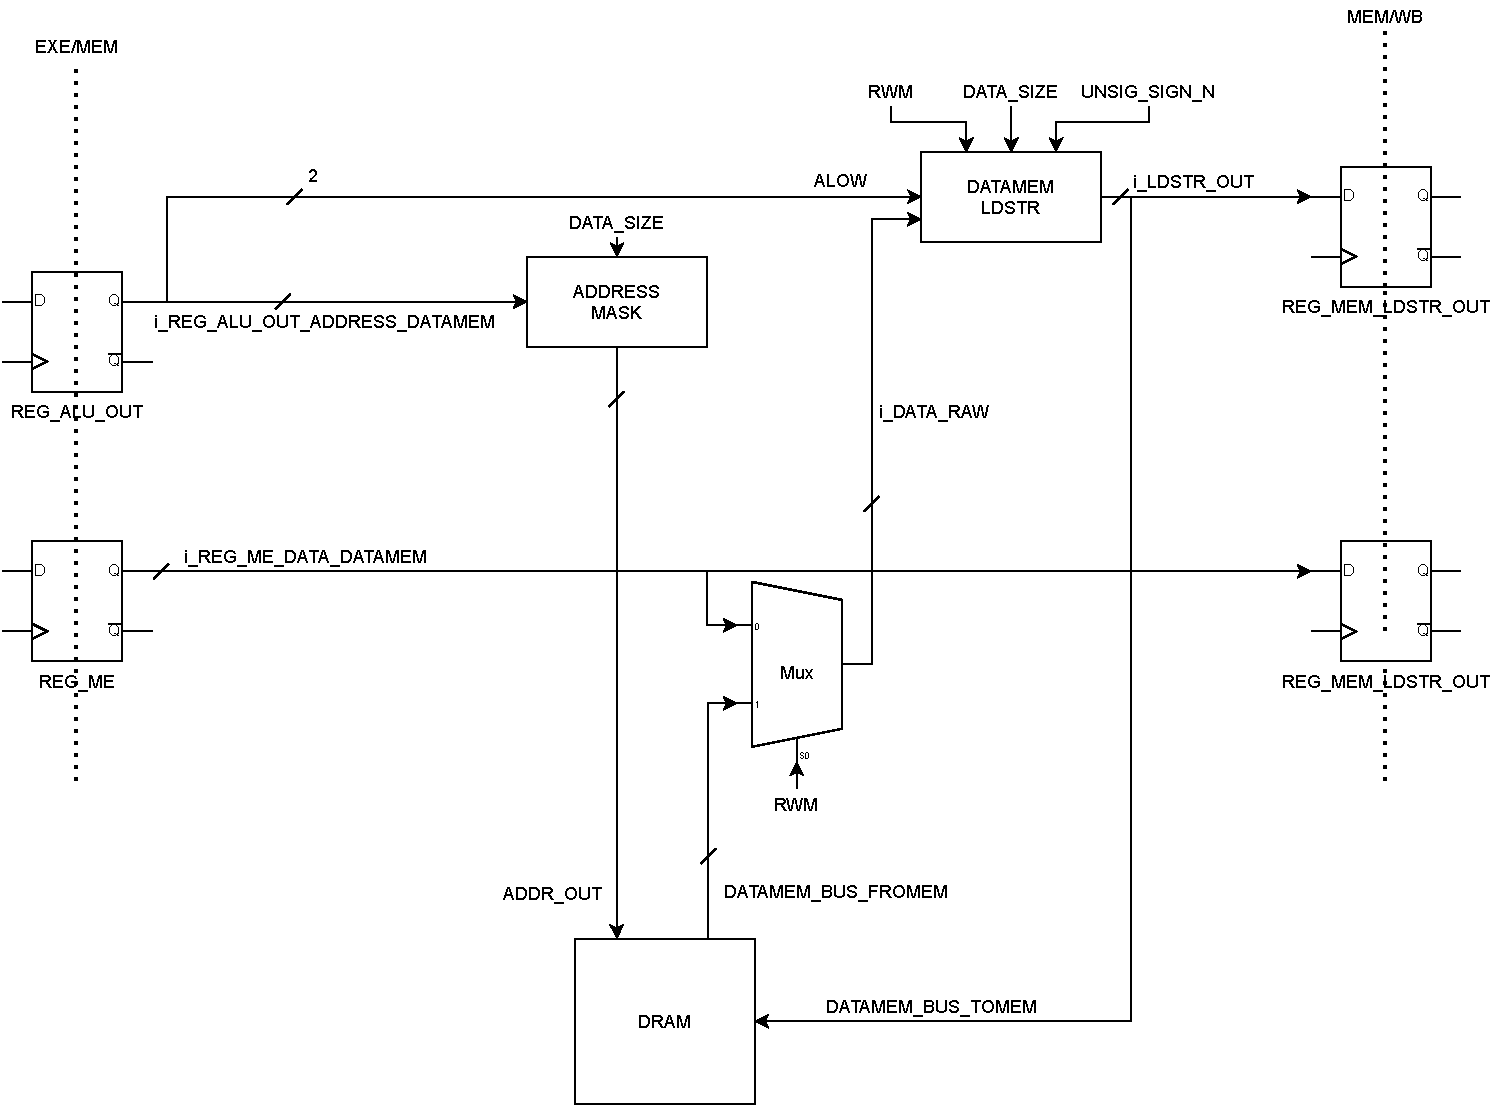
\includegraphics[width=0.85\textwidth]{chapters/6_MemoryStage/images/mem_stage.pdf}
	\caption{Memory stage}
	\label{fig:mem_stage}
\end{figure}

If the instruction that reaches the memory stage is a load, the value stored into the \texttt{REG\_ALU\_OUT} register is fed to a block that performs the masking of the address itself. Then the masked address is given as input to the external memory in order to retrieve the data. A multiplexer with two inputs allows to select the data coming from the memory and redirects it to another unit, called \texttt{datamem\_ldstr} that uses the \texttt{DATA\_SIZE} and \texttt{UNSIG\_SIGN\_N} inputs to select the correct bits for word, half word and byte.

In case of a store, the address in which the data must be saved into the memory is masked too via the Address Mask Unit and its output is given to the DRAM. The data stored in the \texttt{REG\_ME} register is selected, by correctly configuring the multiplex to select it, and put as input to the \texttt{datamem\_ldstr} unit. The output of this unit is put as input data to the DRAM, that perform the store.

\section{Address Mask Unit}
The basic idea behind the Address Mask Unit is to modify the address, given as input, depending on the data size we want to store or load. All the possibility and masking procedures are summed up in the Table \ref{tab:addr_masking}. 

\begin{table}[ht]
	\begin{center}
		\begin{tabular}{ c| l | l}
			\texttt{DATA\_SIZE} & \textbf{Dimension} & \textbf{Masking}\\
			\hline
			00 & word & \texttt{ADDR\_IN(ADDR\_IN'length-1 downto 2) \& "00"}\\
			01 & half word & \texttt{ADDR\_IN(ADDR\_IN'length-1 downto 1) \& "0"} \\
			10 & byte & \texttt{ADDR\_IN}
			
		\end{tabular}
		\caption{Address masking for all the three possible cases}
		\label{tab:addr_masking}
	\end{center}
\end{table}


Give an address, it must be correctly aligned depending on the dimension of the data we want to write/read to/from the memory. Refer to the \ref{vhdl_masking_addr} VHDL snippet. The problem with the alignment arise when data to be accessed are larger that the addressable unit (word vs byte). This allows to read always 32 bits from the memory from the correct position, thanks to the masking process. Since the data is on 32 bits, we need to select 8, 16 or 32 bits from it accordingly to the \texttt{DATA\_SIZE} two bits signal. This is done in the Load-Store Unit.

\hfill
\begin{lstlisting}[style=vhdl,caption={VHDL code for address alignment},label=vhdl_masking_addr]
	with DATA_SIZE select
		ADDR_OUT <= ADDR_IN(ADDR_IN'length-1 downto 2) & "00" when "00",
		ADDR_IN(ADDR_IN'length-1 downto 1) & "0"  when "01",
		ADDR_IN when others;
\end{lstlisting}

\section{Load-Store Unit}
The Load-Store Unit is used to perform two operations:
\begin{itemize}
	\item Extract the correct bits from the data coming from the memory, using the address generated by the Address Mask Unit. Depending of the \texttt{DATA\_SIZE} and the \texttt{ALOW} signals, the data is select.
	
	When the address has been correctly masked in order to fetch a word (32 bits), the data doesn't need to be extracted, neither the sign extension is needed. In the other two cases, when we are managing half word or byte, the correct portion of bits must be taken. 

	\item In case we are managing half word or byte, the bits can be simply taken and set as output of the Load-Store Unit only if we are working with unsigned. In this case, all the others bits are se to 0. On the other hand, if the byte or the half word granularity is used and the \texttt{UNSIG\_SIGN\_N} is set to `0', a sign extension must be performed. In this case, the correct portion of bits is taken, as defined in Table \ref{tab:addr_selection}, and the first bit of it used used extends the sign. 
	\begin{table}[H]
		\begin{center}
			\begin{tabular}{ |c| c | l | l|}
				\hline
				\texttt{DATA\_SIZE} & \texttt{ALOW} & \textbf{Type} & \textbf{Selected bits}\\
				\hline
				00 & * & word & [31-0]\\
				01 & 0* & half A & [31-16]\\
				01 & 1* & half A+2 & [15-0]\\
				10 & 11 & byte A+3 & [7-0]\\
				10 & 10 & byte A+2 & [15-8]\\
				10 & 01 & byte A+1 & [23-16]\\
				10 & 00 & byte A & [31-24]\\
				\hline
				
			\end{tabular}
			\caption{Bits selection using \texttt{DATA\_SIZE} and \texttt{ALOW}}
			\label{tab:addr_selection}
		\end{center}
	\end{table}

	
\end{itemize}
A more detailed explanation of the memory interface is available at section \ref{mas}.